Un problema molto conosciuto e diffuso nelle letteratura relativa al reinforcement learning (RL) è quello del \textit{Cart Pole}.
Esso non è altro che una semplice asta collegata ad un carrello tramite un joint non attuato : questo significa che l'asta risulta essere libera di muoversi, per il semplice fatto che non iruslta essere applicata alcuna azione esterna.
Questo non è altro che un pendolo inverso, ovvero un pendolo che presenta il proprio centro di massa sopra il giunto rotoidale: come si può ben capire dall'immagine in figura ~\ref{fig:CartPole} si tratta di un sistema instabile; infatti, senza un aiuto esterno, il pendolo cadrebbe giù, spostandosi nell'altro equilibrio stabile (ovvero quello ovvio).

\begin{figure}[h]
	\centering
	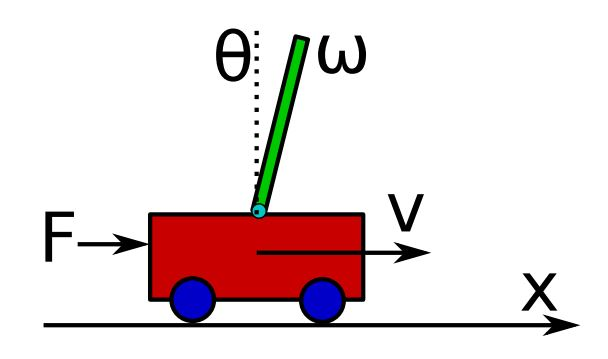
\includegraphics[width=0.5\textwidth]{Immagini/CartPole.JPG}
	\caption{Cart pole e variabili di stato}
	\label{fig:CartPole}
\end{figure}

Il pendolo inverso rappresenta un classico problema relativo alla \textit{dinamica} e alla \textit{teoria del controllo} ed è spesso utilizzato come \textit{problema dummy} per verificare e testare alcune strategie di controllo.
Si capisce quindi che, per mantenere il pendolo inverso nella posizione di equilibrio instabile, risulta essere necessario andare ad applicare una coppia sul punto di giunzione tra l'asta e il carrello, andando a muovere orizzontalmente a destra e a sinistra il carrello.